\documentclass[10pt,aspectratio=169,serif]{beamer}

\usepackage[fontset=none, scheme=plain]{ctex}
\IfFontExistsTF{Songti SC}{%
	\setCJKmainfont{Songti SC}[AutoFakeSlant=0.2]%
	\setCJKsansfont{Songti SC}[AutoFakeSlant=0.2]%
}{%
	\setCJKmainfont{FandolSong-Regular}[Extension=.otf,BoldFont=FandolSong-Bold,AutoFakeSlant=0.2]%
	\setCJKsansfont{FandolSong-Regular}[Extension=.otf,BoldFont=FandolSong-Bold]%
}
\usepackage{amsmath,amssymb,graphicx,tikz,booktabs,multicol,calligra}
\usepackage{pgfplots}
\pgfplotsset{compat=1.18}
\usepackage{tcolorbox}
\tcbuselibrary{skins}
\usepackage{XyygU}
\usepackage{caption}
\captionsetup[figure]{name=图,labelsep=period}

\usetikzlibrary{arrows.meta,positioning,calc}

\setlength{\abovedisplayskip}{0pt plus 2pt minus 2pt}
\setlength{\belowdisplayskip}{0pt plus 2pt minus 2pt}

\title[奇偶性练习]{3.2.2 奇偶性（练习）}
\subtitle{图象对称 \& 定义判定}
\author{}
\institute{}
\date{2026-10-22}

\begin{document}

\begin{frame}
  \titlepage
\end{frame}

% ========== 第1题 ==========
\begin{frame}[t]{第1题：由奇偶性补全图象}
\textbf{1.} 已知 $f(x)$ 是偶函数，$g(x)$ 是奇函数，试将下图补充完整（图中只给出了 $y$ 轴右侧的部分）。

\vspace{0.5em}
\begin{center}
\begin{tikzpicture}[scale=0.9]
% f(x) 右侧
\begin{axis}[
	clip=false,
    width=6cm, height=4cm,
    axis lines=middle,
    xmin=-4, xmax=4, ymin=-1, ymax=3,
    xtick=\empty, ytick=\empty,
    xlabel=$x$,ylabel=$y$,
    xlabel style={below},
]
\draw [magenta,thick](0,0) .. controls (0.5,3) and (2,-1) ..(4,1);
\node[right,magenta] at (axis cs:3.5,1.5) {$f(x)$};
\node[below right] at (0,0) {$O$};
\end{axis}
\end{tikzpicture}
\hspace{1.5cm}
\begin{tikzpicture}[scale=0.9]
% g(x) 右侧
\begin{axis}[
	clip=false,
    width=6cm, height=4cm,
    axis lines=middle,
    xmin=-4, xmax=4, ymin=-2, ymax=2,
    xtick=\empty, ytick=\empty,
    xlabel=$x$,ylabel=$y$,
    xlabel style={below},
]
\draw [magenta,thick](0,0) .. controls (0.5,3) and (2,-1) ..(4,1);
\node[right,magenta] at (axis cs:3.5,0.5) {$g(x)$};
\node[below right] at (0,0) {$O$};
\end{axis}
\end{tikzpicture}
\end{center}
\end{frame}

\begin{frame}[t]{第1题 解答}
\begin{tcolorbox}[colback=orange!10,colframe=orange,title=\textbf{解}]
\begin{itemize}
  \item $f(x)$ 是\alert{偶函数}，图象关于 $y$ 轴对称：将右侧图象沿 $y$ 轴翻折到左侧，得到左半部分。
  \item $g(x)$ 是\alert{奇函数}，图象关于原点对称：将右侧图象绕原点旋转 $180^\circ$（即先关于 $y$ 轴翻折，再关于 $x$ 轴翻折），得到左半部分。
\end{itemize}
\vspace{0.3em}
即：若右侧有点 $(x,y)$（$x>0$），则左侧补上 $(-x,y)$（偶函数 $f$）或 $(-x,-y)$（奇函数 $g$）。
\end{tcolorbox}
\end{frame}

\begin{frame}[t]{第1题 补全后的图象}
\vspace{0.5em}
\begin{center}
	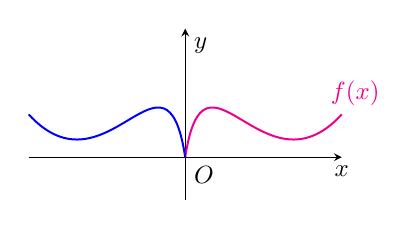
\begin{tikzpicture}[scale=0.9]
		% f(x) 右侧
		\begin{axis}[
			clip=false,
			width=6cm, height=4cm,
			axis lines=middle,
			xmin=-4, xmax=4, ymin=-1, ymax=3,
			xtick=\empty, ytick=\empty,
			xlabel=$x$,ylabel=$y$,
			xlabel style={below},
			]
			\draw [magenta,thick](0,0) .. controls (0.5,3) and (2,-1) ..(4,1);
			
			\draw [blue,thick,](0,0) .. controls (-0.5,3) and (-2,-1) ..(-4,1);
			\node[below right] at (0,0) {$O$};
			\node[right,magenta] at (axis cs:3.5,1.5) {$f(x)$};
		\end{axis}
	\end{tikzpicture}
	\hspace{1.5cm}
	\begin{tikzpicture}[scale=0.9]
		% g(x) 右侧
		\begin{axis}[
			clip=false,
			width=6cm, height=4cm,
			axis lines=middle,
			xmin=-4, xmax=4, ymin=-2, ymax=2,
			xtick=\empty, ytick=\empty,
			xlabel=$x$,ylabel=$y$,
			xlabel style={below},
			]
			\draw [magenta,thick](0,0) .. controls (0.5,3) and (2,-1) ..(4,1);
			\draw [green!40!black,thick,rotate around={180:(0,0)}](0,0) .. controls (0.5,3) and (2,-1) ..(4,1);
			\node[right,magenta] at (axis cs:3.5,0.5) {$g(x)$};
			\node[below right] at (0,0) {$O$};
		\end{axis}
	\end{tikzpicture}
\end{center}
\end{frame}

% ========== 第2题 ==========
\begin{frame}[t]{第2题：判断函数的奇偶性}
\textbf{2.} 判断下列函数的奇偶性：

\vspace{1em}
(1) $f(x)=2x^4+3x^2$；

\vspace{1em}
(2) $f(x)=x^3-2x$。
\end{frame}

\begin{frame}[t]{第2题 解答}
\begin{tcolorbox}[colback=orange!10,colframe=orange,title=\textbf{解}]
(1) 定义域为 $\mathbf{R}$，关于原点对称。
\[
f(-x)=2(-x)^4+3(-x)^2=2x^4+3x^2=f(x).
\]
所以 $f(x)$ 是\alert{偶函数}。

\vspace{0.5em}
(2) 定义域为 $\mathbf{R}$，关于原点对称。
\[
f(-x)=(-x)^3-2(-x)=-x^3+2x=-(x^3-2x)=-f(x).
\]
所以 $f(x)$ 是\alert{奇函数}。
\end{tcolorbox}
\end{frame}

% ========== 第3题 ==========
\begin{frame}[t]{第3题：奇偶性与图象对称的等价关系}
\textbf{3.} (1) 从偶函数的定义出发，证明函数 $y=f(x)$ 是偶函数的充要条件是它的图象关于 $y$ 轴对称；

\vspace{0.8em}
(2) 从奇函数的定义出发，证明函数 $y=f(x)$ 是奇函数的充要条件是它的图象关于原点对称。
\end{frame}

\begin{frame}[t]{第3题 解答 (1)}
\begin{tcolorbox}[colback=orange!10,colframe=orange,title=\textbf{证明 (1)：偶函数 $\Leftrightarrow$ 图象关于 $y$ 轴对称}]
\textbf{必要性：} 若 $f(x)$ 是偶函数，则对任意 $x$，$f(-x)=f(x)$。
这意味着点 $(x,f(x))$ 与点 $(-x,f(x))$ 都在图象上，而这两点关于 $y$ 轴对称，故图象关于 $y$ 轴对称。

\vspace{0.5em}
\textbf{充分性：} 若图象关于 $y$ 轴对称，则图象上任一点 $(x,f(x))$ 关于 $y$ 轴的对称点 $(-x,f(x))$ 也在图象上，即 $f(-x)=f(x)$。故 $f(x)$ 是偶函数。
\end{tcolorbox}
\end{frame}

\begin{frame}[t]{第3题 解答 (2)}
\begin{tcolorbox}[colback=orange!10,colframe=orange,title=\textbf{证明 (2)：奇函数 $\Leftrightarrow$ 图象关于原点对称}]
\textbf{必要性：} 若 $f(x)$ 是奇函数，则对任意 $x$，$f(-x)=-f(x)$。
这意味着点 $(x,f(x))$ 与点 $(-x,-f(x))$ 都在图象上，而这两点关于原点对称，故图象关于原点对称。

\vspace{0.5em}
\textbf{充分性：} 若图象关于原点对称，则图象上任一点 $(x,f(x))$ 关于原点的对称点 $(-x,-f(x))$ 也在图象上，即 $f(-x)=-f(x)$。故 $f(x)$ 是奇函数。
\end{tcolorbox}
\end{frame}

\begin{frame}[c]
  \begin{center}
    {\Huge\calligra Thanks!}
  \end{center}
\end{frame}

\end{document}
